\documentclass[a4paper, 11pt]{report}
\usepackage{changepage}
\usepackage{etoolbox}
\usepackage{fancyhdr}
\usepackage{fancyvrb}
\usepackage[french]{babel}
\usepackage{graphicx}
\usepackage{listings}
\usepackage{pdfpages}
\usepackage[T1]{fontenc}
\usepackage[utf8]{inputenc}
\usepackage{url}
\usepackage{verbatim}
\usepackage{xcolor}
\usepackage{hyperref}

\begin{document}

% configuration du pied de page
\pagestyle{fancy}
\fancyhf{} % efface le style par défaut

% ajout du logo insa (en bas à droite)
\fancyfoot[R]{
\includegraphics[width=1.5cm]{images/logoInsaRouen.jpg}} 
% ajout du numéro de page (en bas au centre)
\fancyfoot[C]{\thepage}

\setlength{\footskip}{20pt}

% correction du style de page des chapitres pour appliquer correctement le pied de page à chacun
\makeatletter
\patchcmd{\chapter}{\thispagestyle{plain}}{\thispagestyle{fancy}}{}{}
\makeatother

% modifie le package hyperref pour eviter les cadre de couleurs autours des hyperliens 
\hypersetup{pdfborder=0 0 0}

% page de garde
\begin{titlepage}

  \centering
  
\includegraphics[scale=0.3]{images/logoInsaRouen.jpg}~\\[0.1cm]
  \textsc{\LARGE Institut National Des Sciences Appliquées}\\[0.1cm]
  \textsc{\LARGE ROUEN NORMANDIE}\\[0.5cm]
  \textsc{\Large Rapport de projet}\\[0.5cm]
  
  {\huge\bfseries Projet intégratif développement orienté objet \par}
  \vspace{0.5cm}

  Étudiants:\\
  \vspace{0.05cm}
  Bonneviale Thomas\\
  El Omari Bouya Lina\\
  Sanson Dylan\\
  Sourdrille Nathan\\

  \vspace{0.5cm}

  Responsables de projet:\\
  \vspace{0.05cm}
  Géraldine Del Mondo\\
  Robin Condat\\
  Nicolas Delestre\\
  Nicolas Malandain\\
  Laurent Vercouter\\
    
    \vspace{2cm}

\date{\today}

\end{titlepage}

\tableofcontents
\pagestyle{fancy}

% === Introduction ===
\section{Introduction}

introduction du rapport



% === Base de Données ===
\chapter{Base de données}

L'objectif de cette partie est d'implémenter la persistance de ITI aventure dans une base de données relationnelle.

% === Compilation ===
\chapter{Compilation}

\section{Organisation}
La partie compilation consistait à créer une version améliorée d'un des lecteurs, le lecteur de fichier texte qui permettait de charger un monde, afin de le rendre plus générique.

Pour cela nous avons appliqué les principes et méthodes appris lors du cours de compilation suivi ce semestre. Nous avons donc décomposé ce sous-projet en différentes parties donc nous avons pu nous occuper en parallèle ou successivement selon les besoins. Le découpage qui a été utilisé est le suivant :

\begin{itemize}
	\item Etude du problème;
	\item rédaction de la grammaire et conformité pour Javacc;
	\item implémentation des classes de l'AST et des classes d'exceptions en Java;
	\item configuration du fichier Javacc;
	\item vérification de la sortie de l'analyseur syntaxique;
	\item implémentation de l'interpréteur (et analyseur sémantique);
	\item implémentation du lecteur et intégration au Main du projet.
\end{itemize}

\section{Etude du problème}
Nous avons commencé cette partie du projet par analyser et comprendre la structure du fichier que nous devions interpréter. Nous disposions d'un exemple sur Moodle ainsi que de la description de chaque mot qui pouvait exister dans ce fichier. Le fichier se présentait de la façon suivante (un extrait seulement) :
\begin{verbatim}
	m1 = monde("LeMondeImpitoyableDeITI")
	bureau_nicos = piece(m1, "BureauDesNicolas")
\end{verbatim}

Une autre contrainte était donnée :  un fichier ne peut créer qu'un seul monde. 

L'objectif final du lecteur étant de créer un monde (et de respecter les contraintes liées à l'interface lecteur), le programme a développé était donc un interpréteur et non un compilateur.

\section{Rédaction de la grammaire}

Notre méthodologie a été itérative, nous sommes partis de l'axiome et avons succesivement créé les éléments donc nous avions besoin pour décrire chaque ligne. Notre grammaire est donc la suivante, l'axiome est ici DeclarationMultiple :
\begin{verbatim}
	DeclarationMultiple -> DeclarationSimple DeclarationSimple*
	DeclarationSimple -> identifiant = Fonction
	Fonction -> nomFonction ( SuiteArguments )
	SuiteArguments -> ArgumentSimple ArgumentSimple*
	ArgumentSimple -> identifiant|chiffre|"chaineDeCaractere"|enumeration|fonction
\end{verbatim}
La grammaire n'étant pas récursive à gauche et ne manipulant pas $\epsilon$ elle est compatible avec Javacc et nous permet donc de passer à l'étape suivante.

\section{Implémentation en Java}
A partir de la grammaire nous avons pu définir la forme que prendrait notre AST et donc définir les classes représentant les noeuds et les feuilles de cet AST : 
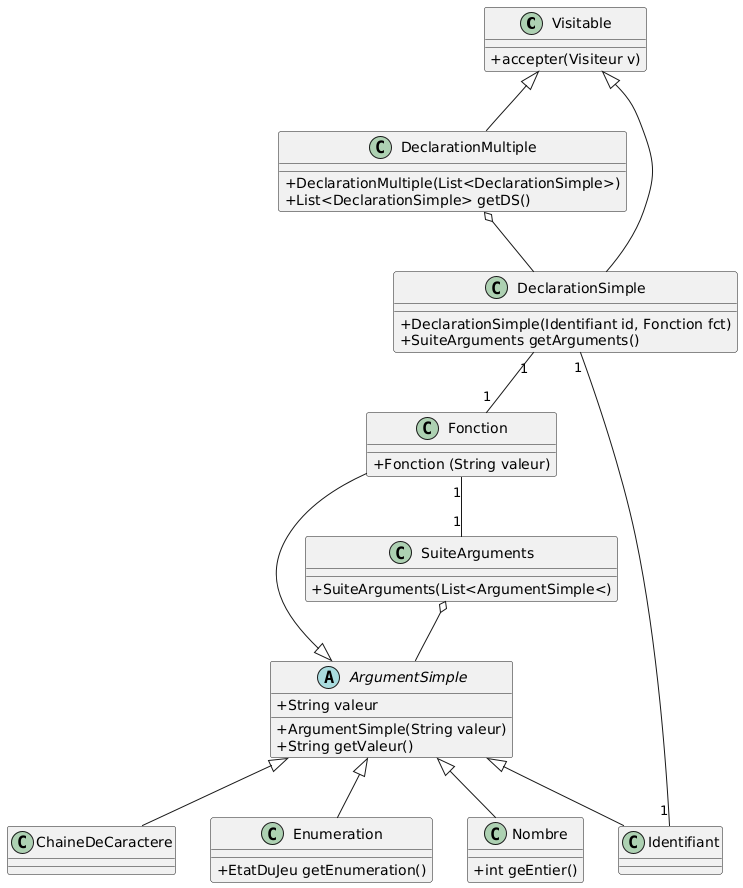
\includegraphics[width=9cm]{images/UML-AST.png}
\\
A partir de là nous nous sommes séparés en deux groupes : un groupe sur l'implémentation en Java et l'autre sur la configuration du fichier Javacc.

Le groupe implémentant les classes en Java a suivi le diagramme de classe définit ci-dessus, ce qui n'a donc pas été très long. Nous avons fait le choix de créer une classe abstraite pour les ArgumentsSimple, ce qui nous a fait implémenter une classe Chiffre et ChaineDeCaractere qui sont des doublons des classes déjà existantes en Java mais qui, selon nous, permettait une meilleure lecture de l'AST.

\section{Configuration du fichier Javacc}
Afin de configurer le fichier Javacc, nous sommes partis de la base du fichier Javacc de la calculatrice présentée lors du cours de compilation. Nous l'avons complété par une SKIP qui permet d'ignorer certains caractères (espaces, sauts de lignes, tabulations, etc.) qui n'ont pas d'intérêt dans la lecture de ce fichier.

Nous avons également transformé les terminaux de la grammaire en expression rationnelle afin de définir les TOKEN qui seront utilisés par l'analyseur lexical.

La dernière partie à consisté à écrire le code Java associé à chaque règle de la grammaire en s'appuyant sur l'implémentation de l'AST définit précédemment par le diagramme de classe. La grammaire étant relativement simple, cette partie a été relativement rapide.

\section{Vérification de l'analyseur syntaxique}
Avant de commencer l'implémentation de l'interpréteur, le groupe qui a implémenté les classes en Java a testé la validité de l'AST produit par l'analyseur syntaxique à partir de quelques lignes du fichier d'exemple. Cette étape nous a permis de nous rendre compte que nous n'avions pas pris en compte les serrures, c'est-à-dire que nous n'avions pas compté qu'une fonction pouvait faire office d'argument (ArgumentSimple) dans une autre fonction. Cela a conduit à une modification de la grammaire, du diagramme de classe et du fichier Javacc. Cette modification n'a heureusement pas induit de changement majeur dans le code. 

Une fois l'AST conforme au fichier de description nous avons pu commencer à implémenter l'interpréteur.

\section{Implémentation de l'interpréteur}
Pour l'interpréteur nous avons fait le choix de le fusionner avec l'analyseur sémantique. La taille du projet permettait une fusion sans que l'implémentation ne soit trop lourde (et sur conseil de M. Delestre).

Une grande partie du temps que nous avons consacré l'interpréteur a consisté à analyser le code des interpréteurs de la Calculatrice et du LightGrep.

Certaines classes qui étaient prévues pour être Visitable n'ont finalement pas été utilisée avec le Design Pattern Visiteur/Visitable, l'accumulation de problème dans le développement de l'interpréteur ne nous a pas permis de suivre correctement l'utilisation de ce Design Pattern.

Les tests de l'interpréteur se sont fait au fur et à mesure de la prise en charge des différentes fonctions du fichier descripteur par l'interpréteur. Cette méthodologie nous a fait gagner un temps précieux.

\section{implémentation du lecteur}
L'interface lecteur nous contraignait simplement à pouvoir récupérer les conditions de fin ainsi que le Monde qui a été chargé. Ce qui nous a poussé à intégrer ces fonctions directement dans l'interpréteur. Ces deux fonctions de l'interpréteur nous ont fait gagner du temps lors du développement du lecteur.

L'implémentation du lecteur s'est effectuée rapidement et sans problèmes majeurs, ce qui nous a permis d'intégrer le lecteur assez rapidement dans le Main du projet et d'avoir un nouveau lecteur fonctionnel.

% === Design-Pattern ===
\chapter{Design Pattern}

Cette partie du projet vise à améliorer la qualité et la réutilisabilité du code ITIAventure en appliquant le Design Pattern Abstract Factory. Ce patron permet de centraliser la création des entités du jeu dans des classes dédiées, tout en facilitant l’extension à d’autres univers sans modifier le code existant.

\section{ITIAventureFactory}

ITIAventureFactory regroupe les méthodes de création des entités de base : Monde, Piece, Porte, Monstre, Serrure, Cle.
Elle encapsule les appels aux constructeurs, ce qui permet de créer des entités sans connaître leur classe concrète.

\section{ITISpaceOperaFactory}

Pour le nouvel univers spatial, nous avons créé ITISpaceOperaFactory, qui hérite de ITIAventureFactory et redéfinit les méthodes de création pour retourner des entités spécifiques : Galaxie, VaisseauSpatial, Teleporteur, Alien, LecteurBadge, Badge.

Grâce à ce système :

    le code principal du jeu reste inchangé ;

    on peut facilement basculer entre les univers ;

    les classes restent ouvertes à l’extension mais fermées à la modification.

\section{Conclusion}

L’usage du pattern Abstract Factory nous a permis de découpler la logique de création des entités du reste du jeu.

% === Conclusion ===
\chapter{Conclusion}

Le projet ITI Aventure nous a permis de mettre en pratique plusieurs compétences acquises durant l’année, en particulier la persistance des données avec JDBC, la création d’un interpréteur via JavaCC, et l’utilisation de design patterns pour améliorer la structure du code.

Nous avons conçu une base relationnelle adaptée au jeu, développé un système de lecture et d’écriture des données en Java, implémenté un langage de description fonctionnel pour créer un monde, et généralisé notre code pour permettre des extensions comme ITISpaceOpera.

Au-delà des aspects techniques, ce projet à développer notre sens de la communication en équipe, à résoudre des problèmes concrets de développement logiciel, et à concevoir une architecture claire et évolutive. Il a constitué une expérience plutôt riche, d'une part par le fait qu'il s'agit du projet informatique le plus concret de l'année et d'autre part car le temps très limité à notre disposition nous contraignait à être prêt pour la date de rendu malgré notamment les contraintes de révision des examens.

\end{document}



